\documentclass[11p]{article}
% Packages
\usepackage{amsmath}
\usepackage{graphicx}
\usepackage{fancyheadings}
\usepackage[swedish]{babel}
\usepackage[
    backend=biber,
    style=authoryear-ibid,
    sorting=ynt
]{biblatex}
\usepackage[utf8]{inputenc}
\usepackage[T1]{fontenc}
\usepackage{titlesec}
\usepackage{hyperref}

%Källor
\addbibresource{references.bib}
\graphicspath{ {./images/} }

% Lite variabler
\def\email{Gabrielnilsson.hogb@elev.ga.ntig.se}
\def\foottitle{}
\def\name{Gabriel Nilsson Högberg}


\begin{document}
    \begin{titlepage}
        \centering

        \vspace*{1cm}

        % Title and subtitle are enclosed between two rules.
        \rule{\textwidth}{1pt}

        % Title
        \vspace{.7\baselineskip}
        {\huge \textbf{Inte tillgänglig för alla}}

        % Subtitle
        \vspace*{.5cm}
        {\LARGE En studie om olika kommunala webbplatsers tillgänglighet}

        \rule{\textwidth}{1pt}

        \vspace{1cm}

        % Set this size for the remaining titlepage.
        \large

        % Authors side by side, using two minipages as a trick.
        \begin{minipage}{.5\textwidth}
            \centering
            Gabriel Nilsson Högberg \\
            {\normalsize \url{Gabrielnilsson.hogb@elev.ga.ntig.se}}
        \end{minipage}%

        \vspace{3cm}

        % Report logo.
        
\includegraphics[width=.7\textwidth]{../images/nti_logo.png}

        \vfill

        % University and date information at the bottom of the titlepage.
        NTI Gymnasiet Umeå \\
        Teknikprogrammet\\
        Gymnasiearbete\\
        Datum: \today \\
        Handledare: Jens Andreasson
    \end{titlepage}

    \tableofcontents

% i Sverige har vi normalt inget indrag vid nytt stycke
    \setlength{\parindent}{0pt}
% men däremot lite mellanrum
    \setlength{\parskip}{10pt}

    
    \section{Inledning}
    Webben som vi känner till idag har blivit en av världens mest använda verktyg sedan det släpptes för allmänheten i 1993.
    I världen är det runt 4,39 miljarder personer som använder sig av internet vilket är över hälften av den globala populationen \textcite{history_WWW}.
    I Sverige är det runt 95 procent som använder sig av internet \textcite{SCB} och att så många personer använder internet ställer allt större krav på att webbplatserna ska fungera så att alla kan använda dem på ett bekvämt sätt.
    Detta gör även att det ställs ett större krav på att webbsidorna ska vara tillgängliga.
    Ett stort ansvar hamnar då på kommunala webbsidor att webbplatsen ska vara tillgänglig oavsett vilken enhet man använder.
    Ett extremt stort spektrum av behov behövs täckas för att kalla en webbsida tillgänglig.

    Den svenska myndigheten för digital förvaltning (DIGG) ger denna anledning till varför fokuset på tillgänglighet är viktigt:

    ``Omkring 16 procent av den globala befolkningen uppskattas att ha en signifikant funktionsnedsättning och denna siffra fortsätter att öka bland annat med åldrande befolkning.
    För personer med funktionsnedsättning kan god tillgänglighet vara helt avgörande för att kunna ta del av information eller utföra ett ärende på en offentlig webbplats \textcite{Digg_tillganglighet}.
    ``

    World Wide Web Consortium (W3C) arbetar med att förbättra Web content accessibility guidelines (WCAG) för att ge en standard om tillgänglighet på webben och för webbutvecklare.
    Många använder sig av denna standard för att skapa sin egna sida från ett tillgänglighets perspektiv.
    Jag anser att det skulle vara intressant att undersöka svenska kommunala webbsidor och ifall dem följer tillgänglighetsstandarderna WCAG 2.0 och 2.1 och jämföra dem med andra kommuners webbsidor.
    
    \section{Syfte och Frågeställning}
    Undersökningen kommer att ta reda på hur sidorna möter kriterier samtidigt som prestanda, tillgänglighet och bästa praxis kommer att mätas med hjälp av ett antal automatiserade tester.

    Syftet för själva undersökningen och varför detta är viktigt att undersöka är för att ge så många som möjligt möjligheten att kunna använda internet på ett tillräckligt bra sätt utan att utsättas för onödiga svårigheter.
    Detta är speciellt viktigt för de offentliga webbsidorna.

    I denna undersökning kommer följande sidor att undersökas:

    \begin{itemize}
        \item eslov.se
        \item goteborg.se
        \item helsingborg.se
        \item huddinge.se
    \end{itemize}

    Utifrån dessa frågeställningar:

    \begin{itemize}
        \item Möter webbsidan tillgänglighetskriterier som står i WCAG 2.0 och 2.1?
        \item Vilka kriterier misslyckades webbsidorna mest med?
        \item Vilken prestanda, tillgänglighet och hur god praxis följer webbsidorna.
    \end{itemize}
    
    \section{Bakgrund}
    
    \subsection{Vad är webbtillgänglighet?}
    Tillgänglighets aspekter kan skilja från person till person men vad exakt tillgänglighet är kan vara svårt att sätta fingret på men för denna studie används Steve Krug och hans egna definition av webbtillgänglighet i sin bok Don't Make Me Think revisited: A Common Sense Approach to Web Usability \textcite{Krug}.
    Steve Krug är ett UX-proffs som är känd för sin bok "Don't Make Me Think" som handlar om interaktionen mellan människa, dator och användarvänligheten på webben \textcite{Krug_Wikipedia}.
    Krug leder även ett enmanskonsultföretag som heter Advanced Common Sense.

    Det är inte bara Steve Krug som tänker på detta sätt utan Jakob Nielsen som är konsult inom dator- och webbanvändbarhet som anses vara en av de ledande auktoriteterna inom användbarhet tänker på ett likvärdigt sätt \textcite{Jakob_Nielsen}.
    Han är känd för sin hård kritik mot populära webbplatser och mot överdriven användning utav grafik och animeringar som inte hjälper användbarheten.
    Nielsens tio heuritiska principer liknar de punkter som Krug har gjort för sin egna bok.

    Steve Krug och hans egna definition av användbarhet är följande:


    ``Du kommer hitta olika definitioner av användbarhet men ofta bryts det ned i olika punkter som;``

    \begin{itemize}
        \item Användbar: Gör den något som användaren behöver?
        \item Lärbar: Kan användaren lära sig hur man använder detta?
        \item Minnesvärd: Behöver användaren lära sig om denna sak varje gång den används?
        \item Effektiv: Får den jobbet gjort på en rimlig tid med den insats som denna användare gör?
        \item Önskvärd: Vill användaren ha detta?
        \item Trevlig: Tycker användaren att detta är trevligt eller till och med roligt att använda?
    \end{itemize}

    När något är användbart ska alltså en person som har erfarenheter och förmågor kunna lista ut hur man använder en produkt utan att det ska ta för mycket tid och energi än vad som egentligen behövs.

    \subsection{Alt-Taggar}
    En alt-tagg är en alternativ text till img element på en webbsida och ska förklara och ge kontext till vad den är kopplad till.
    Ett bra exempel för detta är text som kan berätta vad som är på bilden och ge kontext varför den är här på sidan \textcite{Nordström}.

    \subsection{WAI-ARIA}
    WAI-ARIA används för att göra webbinnehåll mer tillgängligt för personer som använder hjälpmedel som skärmläsare och har blivit en teknisk standard. \textcite{ARIA}
    Problemet med WAI-ARIA är att det oftast används felaktigt och gör en webbsida mer otillgänglig istället eftersom personer med hjälpmedel ska kunna ta en del av webbplatser används ARIA-attribut som stöd i HTML-kod.
    Med korrekt användning av WAI-ARIA kan en webbläsare översätta HTML-kod till en skärmläsare som i sin tur läser upp för användaren om till exempel en meny är öppen eller stängd \textcite{7minds}.


    \subsection{Kontraster}
    Ett av de vanligare felen som kan uppstå på webbsidor är dåliga kontraster.
    Olika kontrastfel uppstår då det är svårt att se innehållet på grund av färgerna på webbsidan.
    Detta kan vara en text som inte syns på grund av att bakgrundsfärgen har för dålig konstrast jämfört med själva texten.
    Detta gör att ett stort problem uppstår speciellt för de som har synnedsättning eller nedsatt färgseende \textcite{Digg_2021}.
    Exempel på kontrastfel syns nedan i figur 1.

    \begin{figure}[hbt!]
        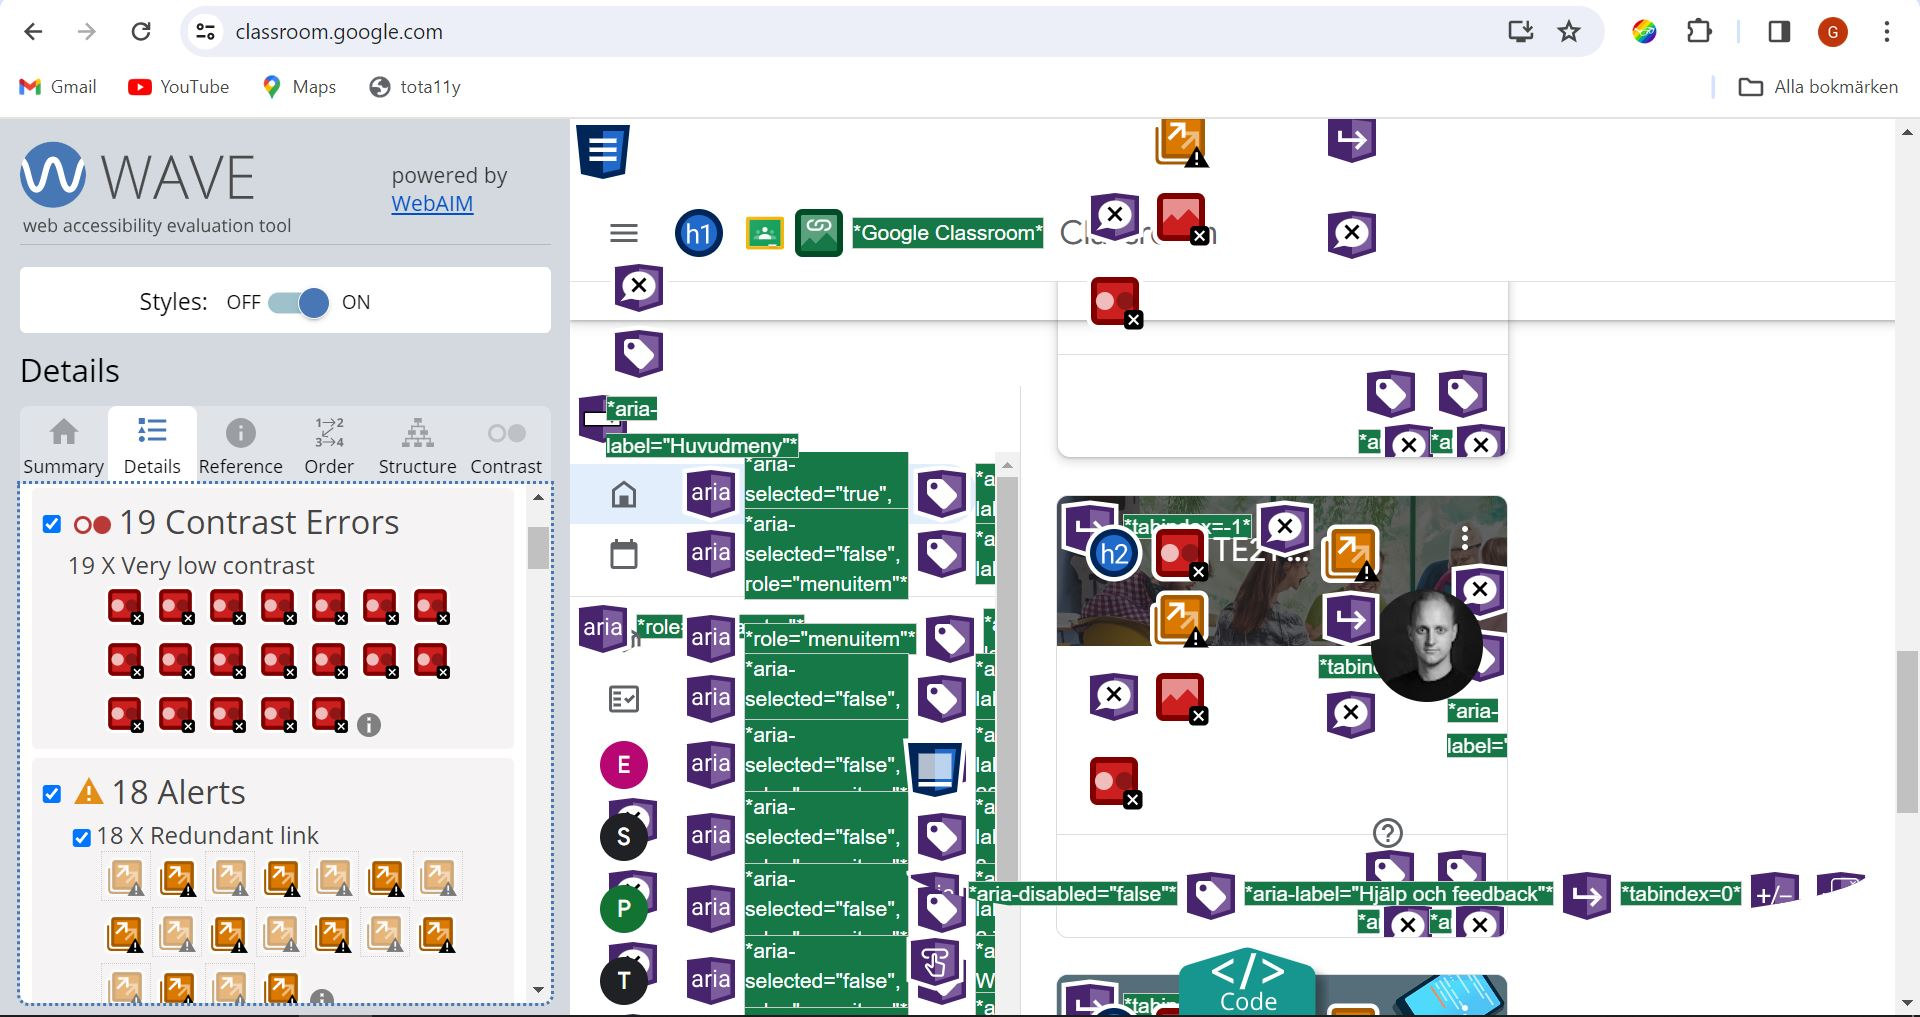
\includegraphics[width=0.8\textwidth]{../images/KontrastExempel.jpg}
        \caption{ Kontrastexempel 1 }
    \end{figure}

    \section{Vad är World Wide Web Consortium? (W3C)}
    World Wide Web Consortium även förkortat till W3C skapades av Tim Burners-Lee och arbetar med att skapa en webb som är tillgänglig för alla.
    W3C skapar och utvecklar olika webbstandarder för att uppnå detta.
    W3Cs egna dokument om Web Content Accessibility Guidelines har blivit standarden inom webbutvecklings industrin \textcite{W3C}.

    \subsection{Vad är Web Content Accessibility Guidelines? (WCAG)}
    Web Content Accessibility Guidelines är ett dokument gjort av W3C som har riktlinjer på hur vi ska göra webben tillgänglig för så många som möjligt.
    W3C beskriver själv vilka områden som WCAG ska behandla:

    ``Genom att följa dessa riktlinjer kommer innehållet att bli mer tillgängligt för en större andel av personer med funktionsnedsättning, inklusive hjälpmedel för blindhet och nedsatt syn, dövhet och hörselnedsättning, begränsad rörelse, talsvårigheter, ljuskänslighet och kombinationer av dessa, och vissa hjälpmedel för inlärningssvårigheter och kognitiva begränsningar; men kommer inte att tillgodose alla användarbehov för personer med dessa funktionshinder.`` \textcite{WCAG}

    WCAG har även olika krav som indelas i möjlighet att uppfatta, hanterbarhet, begriplighet och hur robust en sida är.
    Möjlighet att uppfatta innehåller att en person ska kunna uppfatta sidan och att innehållet ska kunna presenteras på olika sätt som t.ex text kan konverteras till större stil.
    Hanterbarhet innebär att sidan ska kunna navigeras utan mus, alltså med tangentbord eller andra hjälpmedel.
    Begripligheten för sidan ska vara att det finns inmatningsstöd som hjälper användaren undvika eller rätta till misstag.
    Till sist ska sidan vara robust, innehållet ska vara robust för ett brett spektrum av användarprogram inklusive hjälpmedel som skärmläsare.
    Alla dessa krav tillsammans gör att en sida kan vara så användarvänlig och tillgänglig för dem flesta personerna. \textcite{Digg_2023}

    \subsection{Vad är Webb Accessibility Initiative? (WAI)}
    WAI är ett initiativ från W3C som är till för att öka prioriteten för användbarhet för dem med funktionsnedsättningar.
    Initiativet utvecklas genom att arbeta med olika industrier, organisationer, regeringar och mer för att runt om i världen göra webben mer tillgänglig.
    WAI har några primära aktiviteter som:

    \begin{itemize}
        \item Garantera att W3C standarder utvecklas med tankar för tillgänglighet
        \item Utveckla tillgänglighets riktlinjer för webben och appar
        \item Utveckla resurser för att förbättra webbtillgänglighets utvärderingar
        \item Fortsätta lära ut om webbtillgänglighet
        \item Samarbeta med undersökningar och andra utvecklingar som kan påverka webbtillgänglighet i framtiden
        \item Påverka fler att tänka på webbtillgänglighetsstandarder
    \end{itemize}

    \textcite{WAI}

    \subsection{Testverktyg}

    \begin{itemize}
        \item AChecker
        \item WAVE
        \item Lighthouse
    \end{itemize}

    \subsection{AChecker}
    AChecker är ett tillgänglighetsverktyg som Web Accessibility Initiative (WAI) beskriver som.

    "Interaktiv, internationell och justerbar webbtillgänglighetsgranskare.
    AChecker tillåter användare att göra sina egna riktlinjer och bearbeta sina egna tillgänglighets granskningar.
    Detta är baserat på Open Accessibility Checks (OAC)" \textcite{AChecker}

    AChecker använder olika riktlinjer och standarder för att kontrollera att en webbsida möter dessa standarder och riktlinjer som testet använder sig av.
    Efter att verktyget granskat webbsidan presenteras resultat i tre olika nivåer.

    \begin{itemize}
        \item Kända problem: Problem som programmet hittar och vet är fel på webbsidan
        \item Sannolika problem: Problem som kan vara fel men behövs kollas manuellt
        \item Potentiella problem: Problem som programmet inte själv kan förstå eller hantera och måste också manuellt kollas ifall det verkligen är ett fel.
    \end{itemize}
    
    \subsection{Web Accessibility Evaluation Tools (WAVE)}
    Web Accessibility Evaluation Tools (WAVE) är ett tillgänglighetsverktyg som går att lägga till i chrome som en extension.
    WAVE skapades 2001 av Webb Accessibility In Mind (webAIM) i Utah State University \textcite{WAVE}.
    Programmet i sig använder sig av WCAG som riktlinjes standard och som webbsidorna testas på.
    WAVE är även uppskriven i WAI tillgänglighetsprogram listan som rekommenderas att använda.

    \subsection{Lighthouse}
    Lighthouse är gjort av Google och är ett verktyg till för att undersöka webbsidor i fem olika kategorier och sedan lägger ett betyg på en skala mellan 0 - 100.
    Det fem olika kategorierna som undersöks av lighthouse är: prestanda, tillgänglighet, bästa praxis, sökmotoroptimering (SEO) och progressiv webbapp.
    Man får även kommentarer och sedan säger den till om vad som är fel med någon av dessa fem olika kategorier.
    
    \subsection{Sveriges arbete med tillgänglighet}
    Sveriges arbete med tillgänglighet på webben baseras på de lagar som Sverige använder sig av.
    Lagen om Digital offentlig Service (DOS-lagen) handlar om att den offentliga sektorn följa denna lag.
    För att kunna uppnå kraven som DOS-lagen innehåller rekommenderar DIGG att följa den europeiska standarden EN 301 549 som hänvisar till WCAG 2.1 på AA nivå \textcite{Digg_Dos}.
    Däremot rekommenderas det att en webbsida ska uppnå kraven till AAA nivå.
    EN 301 549 innehåller alltså fler kriterier som ska följas av offentliga webbsidor.

    \section{Metod}
    Tillgänglighetsstandarden idag har utökats enormt och förbättrar användarupplevelsen för alla.
    Inom Sverige har vi WCAG som riktlinjer och webbsidor bör följa och även uppnå de krav som riktlinjerna ger \textcite{Digg}.
    Det är för allas bästa att dessa används för att förbättra sina och andras webbsidor så att alla kan använda dem.

    \begin{itemize}
        \item Med hjälp av programmet AChecker går det att kontrollera en webbsida på WCAG 2.0 kraven och alla tre nivåer A, AA och AAA. Dessa nivåer anger ambitionsnivån på sidan och grunden för tillgänglighetskrav är AA.
        \item Ett manuellt test kommer att göras för att utöka kraven till WCAG 2.1, alltså krav som inte står i WCAG 2.0 med hjälp av WAVE.
        \item Det manuella testet kommer att undersöka ifall ARIA-referenser fungerar och om det finns alt-taggar på bilder, loggor och mer.
        \item Lighthouse kommer att användas för att kolla sidornas prestanda, tillgänglighet och praxis.
    \end{itemize}

    För att undvika mänskliga misstag under undersökningen används utvärderingsverktyg.
    Det manuella testet kommer att göras eftersom det inte finns tillräckligt bra verktyg som kontrollerar WCAG 2.1 kriterierna.
    WAVE kommer att användas för att effektivisera manuella undersökningen med kontraster, ARIA-referenser och alt-taggar.
    Till sist kommer Lighthouse användas för att hitta problem som inte kan hittas av utvärderingsverktyg eller den manuella kontrollen.

    \subsection{Val av sidor}
    Sidorna som valdes för denna undersökning är:

    \begin{itemize}
        \item eslov.se
        \item goteborg.se
        \item helsingborg.se
        \item huddinge.se
    \end{itemize}

    \subsection{AChecker}
    AChecker är en rekommendation från \textcite{AChecker} och används som en av tillgänglighets programmen för webbutvecklare.
    Programmet underlättar undersökningen av kraven inom WCAG 2.0 på alla tre nivåer A, AA och AAA.

    \subsection{Lighthouse}
    Sidorna som testas kommer köras 3 gånger med lighthouse för att få så bra data som möjligt på webbsidorna.
    Appar och annat kommer stängas av för att inte påverka och ifall något program är igång kommer det att skrivas ned.
    Sidorna körs två gånger för att kontrollera om det uppstår någon skillnad i resultaten.

    \subsection{Det manuella testet}
    Det manuella testet kommer att undersöka WCAG 2.1 eftersom programmen använt hittills inte täcker de kraven som står där.
    Därför kommer WAVE användas för att kolla ARIA-referenser, kontraster och sidornas kodstruktur.

    \subsection{Alt-taggar}
    För att undersöka alt-taggar kommer DevTools (inspektor) användas för att se till att html koden innehåller alternativ text till bilder och att dem stämmer men också knappar med namn och att deras namn också stämmer.

    \subsection{Analysering}

    Allt data som insamlas kommer att jämföras och analyseras med riktlinjerna i både WCAG 2.0 och 2.1.
    Detta görs för att se om webbsidorna följer dessa riktlinjer eller inte.

    \section{Resultat}
    
    \subsection{WCAG 2.0 och 2.1}
    Det mest vanliga kriteriet som webbsidorna inte når upp till är 1.1.1.
    Kriteriet förklarar att alternativ text ska finnas på bilder.
    Det andra kriteriet som inte webbsidorna häller når upp till är 2.5.3 som innebär att all inmatningselement med text eller bild ska ha likadana namn, detta gör att det blir enklare att använda röstinmatning.
    Till sist är det kriterium 2.4.6 som innebär att rubriker och etiketter för formulär och interaktiva kontroller ska vara informativa.
    Antalet gånger som webbsidorna misslyckades med dessa kriterier syns i figur 2.

    \begin{figure}[hbt!]
        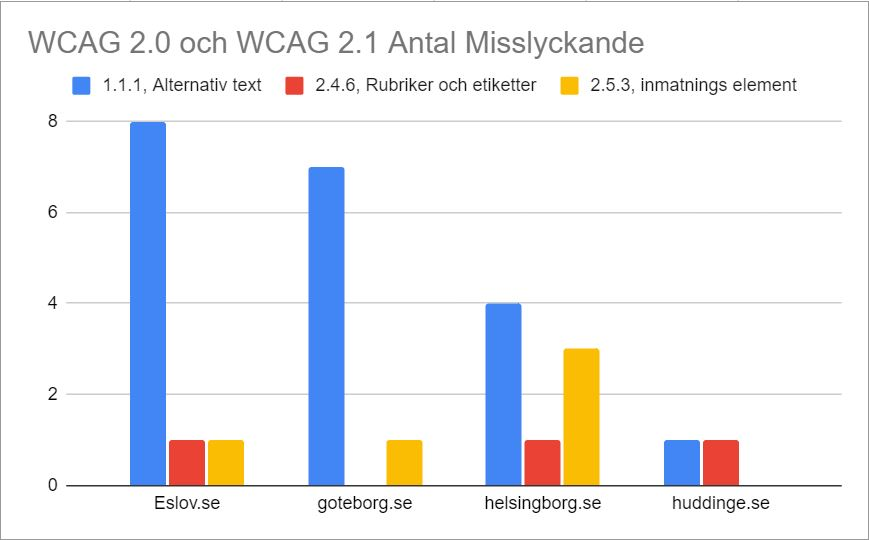
\includegraphics[width=0.8\textwidth]{../images/antalmisslyckande.jpg}
        \caption{ Antal misslyckande på kriterier }
    \end{figure}

    \subsection{Analysering}
    
    \subsubsection{Kriteriet 1.1.1, Alternativ text}
    Kriteriet 1.1.1 hanterar allt innehåll som inte är text och om det finns på sidan ska den ha ett textalternativ.
    Innehållet som kategoriseras i kriteriet 1.1.1 är följande:

    \begin{itemize}
        \item Bilder som är aktiva på sidan
        \item Interaktiva bilder
        \item Informativa bilder
        \item CSS bilder
        \item Dekorativa bilder
        \item Komplexa grafer och diagram
        \item Kartor
        \item Inmatningskontroll bilder (t.ex en knapp som ser ut som en bild istället för att ha text)
        \item CAPTCHA (Completely Automated Public Turing test to tell Computers and Humans Apart)
        \item Ljud och video innehåll
    \end{itemize}

    Efter analyseringen av webbsidornas resultat så visade det sig att alla webbsidor inte klarade av detta kriteriet eftersom det var minst ett misslyckande per sida.
    Bilderna som orsakade att detta kriteriet inte uppnåddes hade inte fullständiga alternativa texter eller text runt om som kunde förklara bilderna.
    Resultatet efter denna analys är; eslov.se 8 misslyckande, goteborg.se 7, helsingborg.se 4 och huddinge.se 1.
    Nedan är bilder på webbsidorna där det syns vad exakt som misslyckades och detta syns i figurerna 3 och 4

    \begin{figure}[hbt!]
        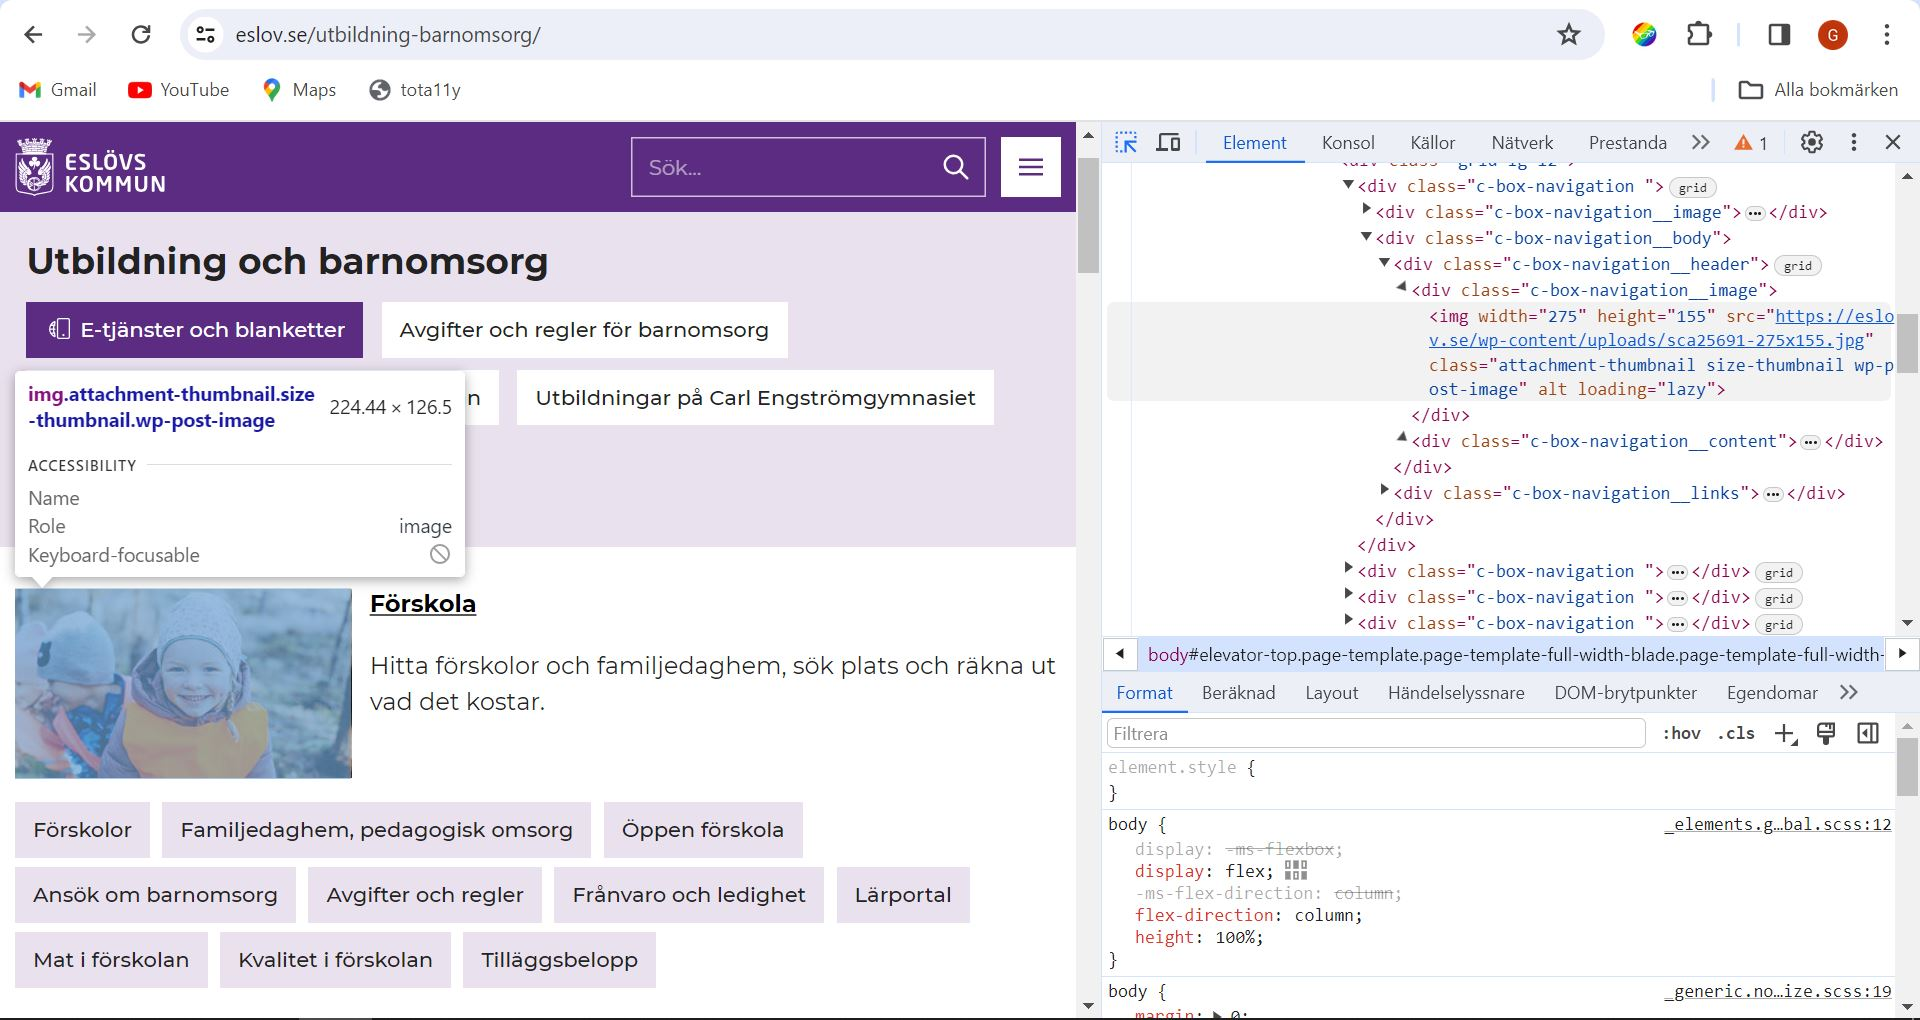
\includegraphics[width=0.8\textwidth]{../images/Eslov111.jpg}
        \caption{ Eslov.se misslyckande av kriteriet 1.1.1 }
    \end{figure}

    \begin{figure}[hbt!]
        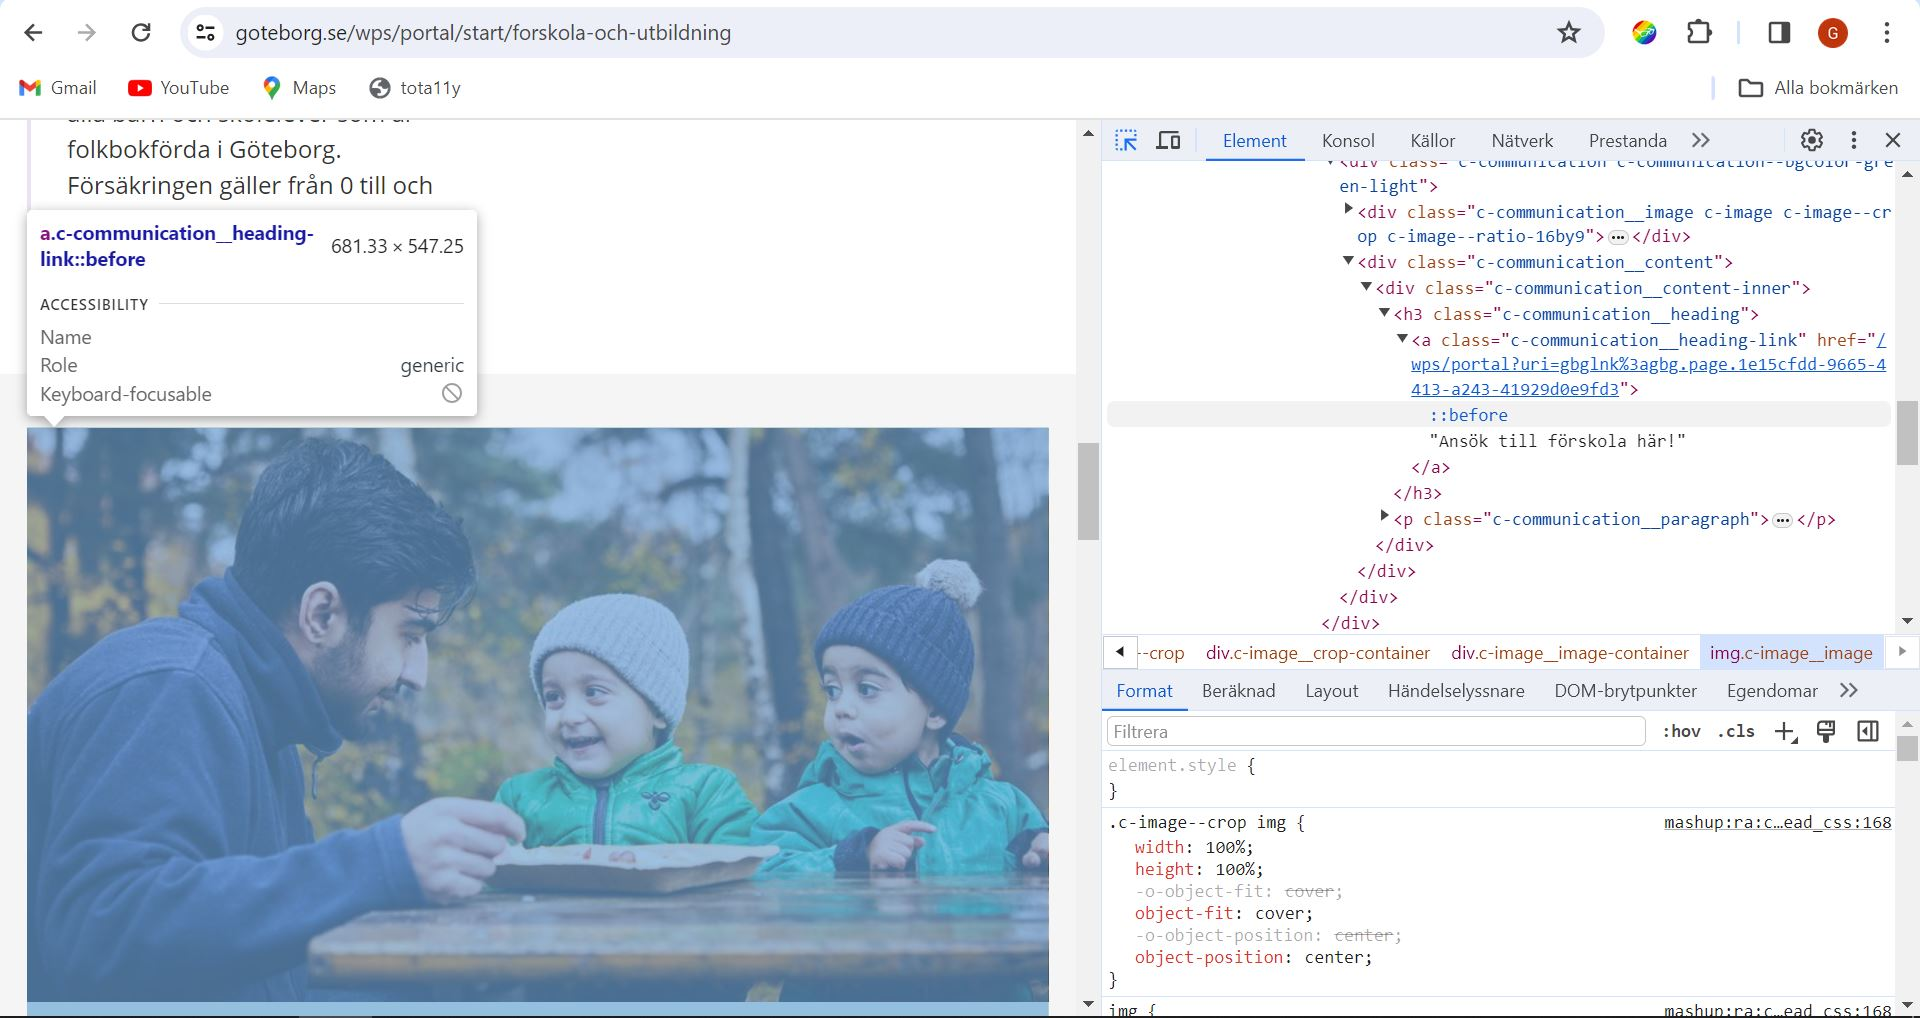
\includegraphics[width=0.8\textwidth]{../images/Goteborg111.jpg}
        \caption{ Goteborg.se misslyckande av kriteriet 1.1.1 }
    \end{figure}

    \subsubsection{Kriteriet 2.4.6, Rubriker och etiketter}
    Kriteriet 2.4.6 hanterar innehåll som rubriker eller etiketter på en webbsida och om detta finns ska dem vara informativa eftersom detta hjälper de som använder sig utav skärmläsare och hoppar mellan rubriker.
    Detta kriteriet involverar inte att man ska använda sig utav rubriker och etiketter utan bara om de används ska de användas på rätt sätt, skrivna tydligt och meningsfullt.

    Efter analyseringen av webbsidornas resultat visade det sig att goteborg.se klarade av detta kriterier, samt tas bort från deras resultat
    goteborg.se har rubriker och etiketter som är skrivna tydligt och är meningsfulla.
    Eslov.se och huddinge.se har en rubrik som inte har någon text vilket gör att den inte är tydlig eller meningsfull.
    Helsingborg.se har en etikett till ett formulär som saknar en meningsfull text som gör att skärmläsare inte kan visa denna information korrekt.
    Rubrikerna och etiketterna som orsakade att detta kriteriet inte uppnåddes hade icke fullständiga rubriker och etiketter som inte var tillräckligt tydliga eller meningsfulla.
    Resultatet efter denna analys är; goteborg.se 0 misslyckande, eslov.se 1, huddinge.se 1 och helsingborg.se 1.
    Nedan syns bilderna ifrån de webbsidorna som misslyckade med kriteriet och detta är figurerna 5, 6 och 7.

    \begin{figure}[hbt!]
        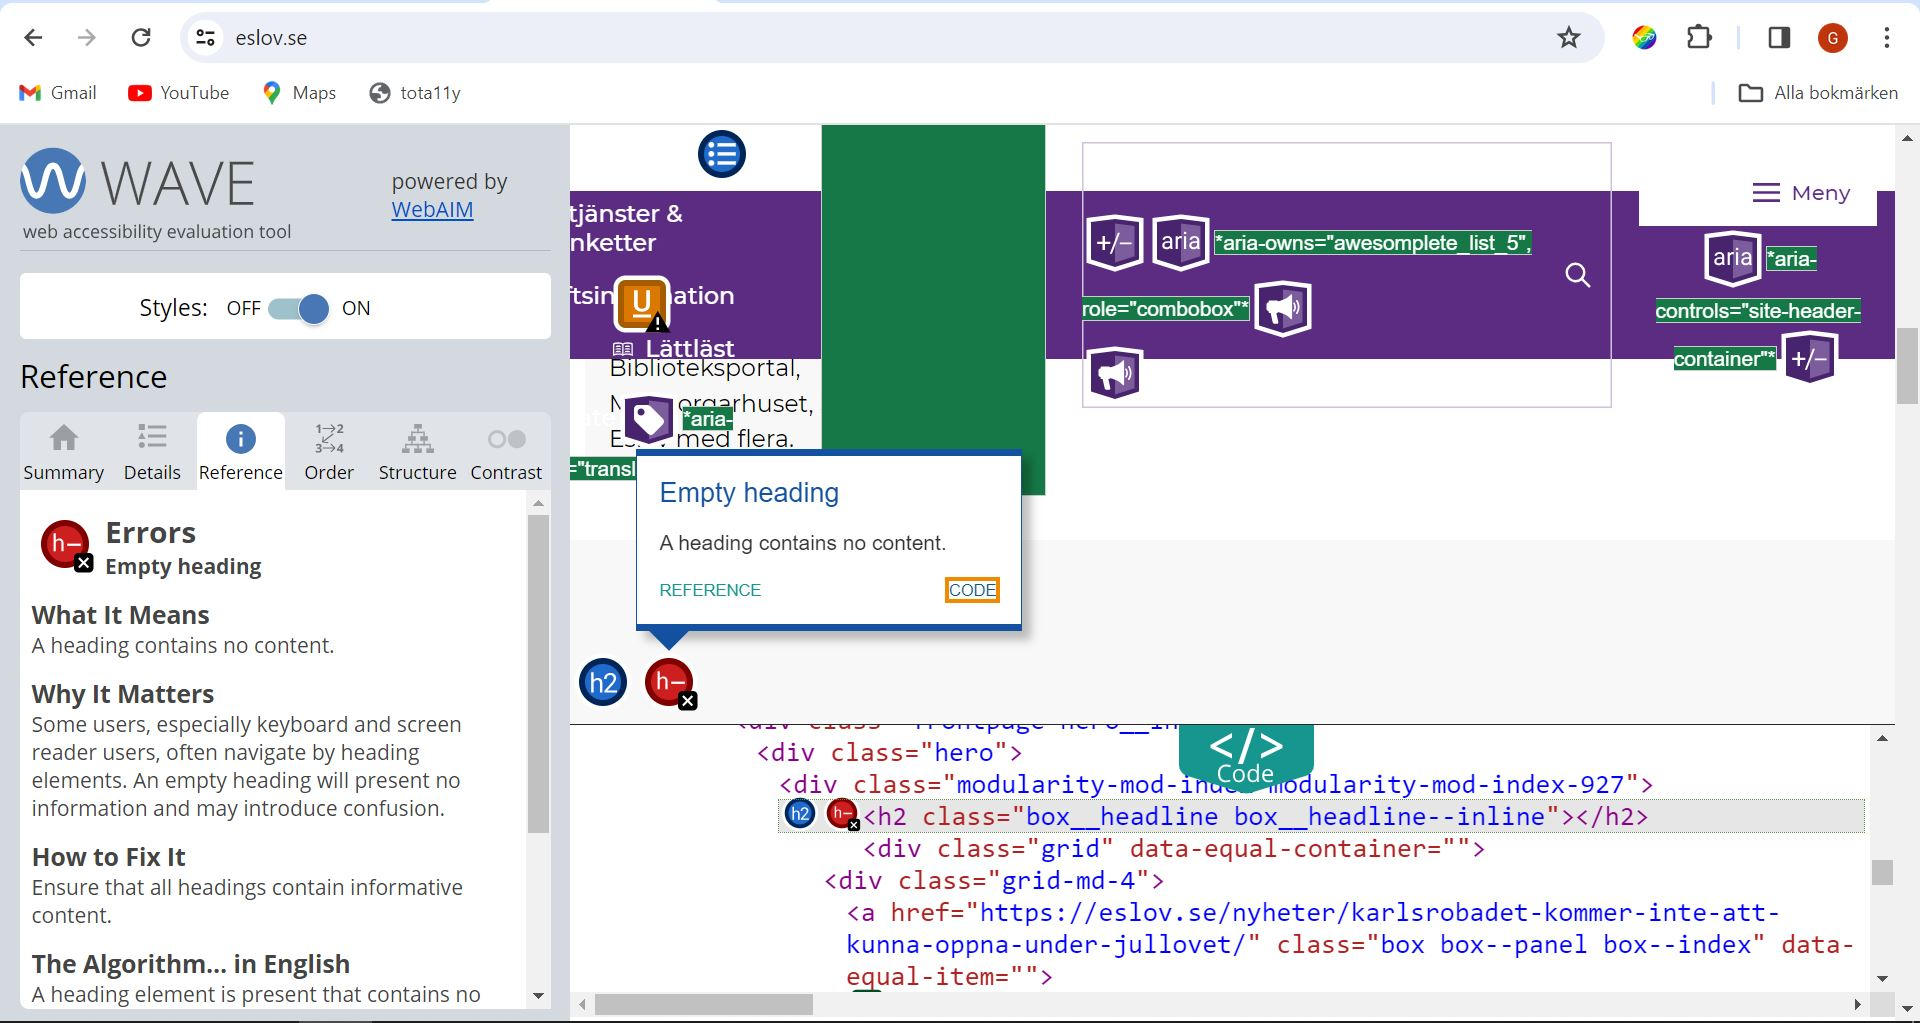
\includegraphics[width=0.8\textwidth]{../images/Eslov246.jpg}
        \caption{ Eslov.se misslyckande av kriteriet 2.4.6 }
    \end{figure}

    \begin{figure}[hbt!]
        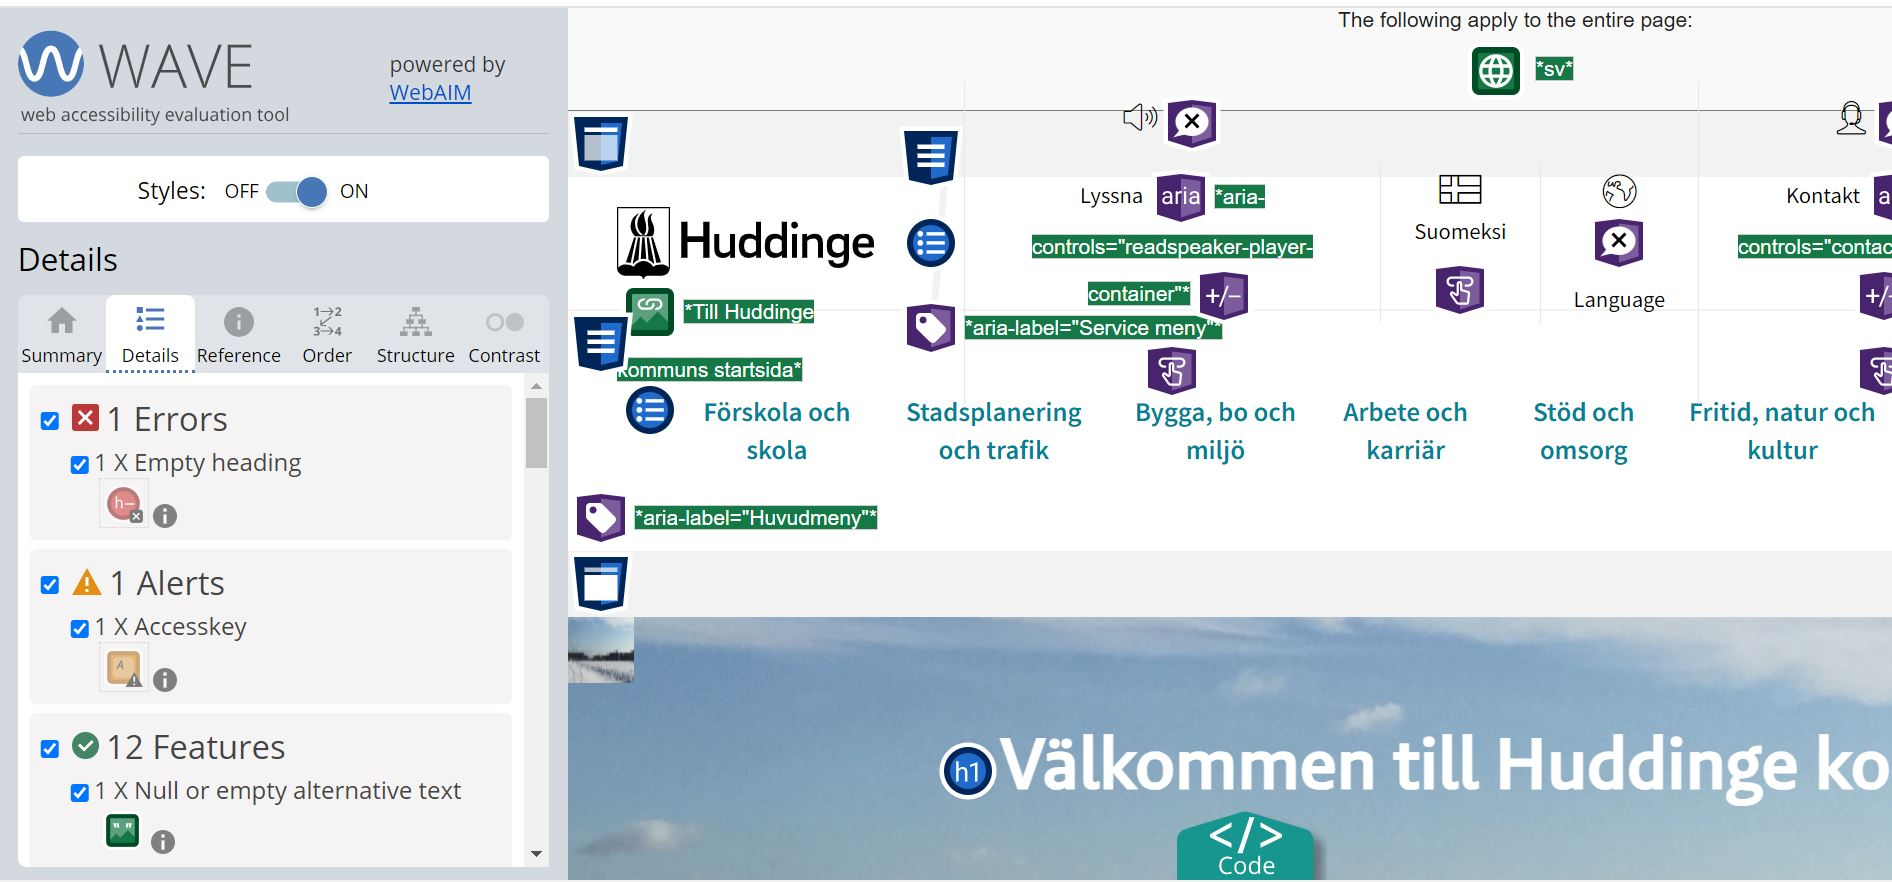
\includegraphics[width=0.8\textwidth]{../images/Huddinge246.jpg}
        \caption{ Huddinge.se misslyckande av kriteriet 2.4.6 }
    \end{figure}

    \begin{figure}[hbt!]
        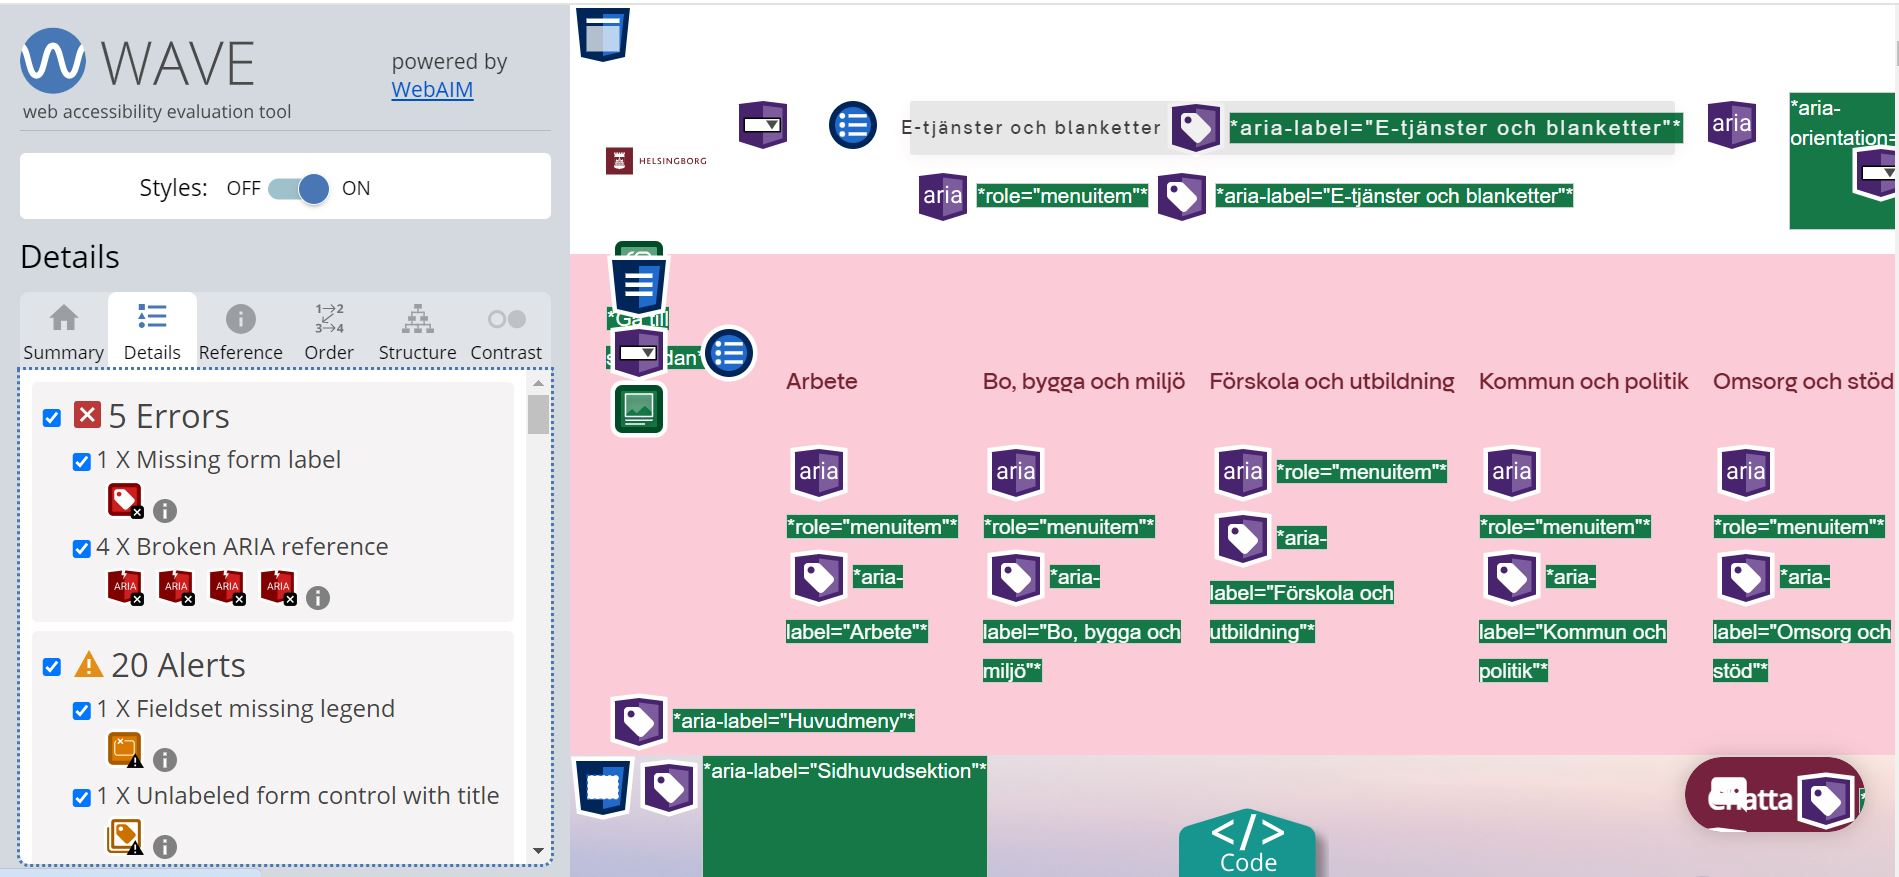
\includegraphics[width=0.8\textwidth]{../images/Helsingborg246.jpg}
        \caption{ Helsingborg.se misslyckande av 2.4.6 }
    \end{figure}

    \subsubsection{Kriteriet 2.5.3, Inmatningselement}
    Kriteriet 2.5.3, hanterar innehåll som interaktiva element som till exempel knappar.
    Dessa element ska ha en alternativ etikett eller så måste etiketten ha samma namn som texten på elementet, detta är för att röstinmatning ska kunna hitta elementen.
    Om etiketten inte är detsamma som texten blir det svårt att använda röstinmatning för att navigera webbsidor.

    Exempel kommer att visas från varje sida som inte uppfyllde kriteriet och sedan kommer det förklaras varför i figurens bildtext.
    eslov.se, helsingborg.se och goteborg.se hade felet att namnet på knapparna är fel som visas i figurer 8, 9 och 10

    \begin{figure}[hbt!]
        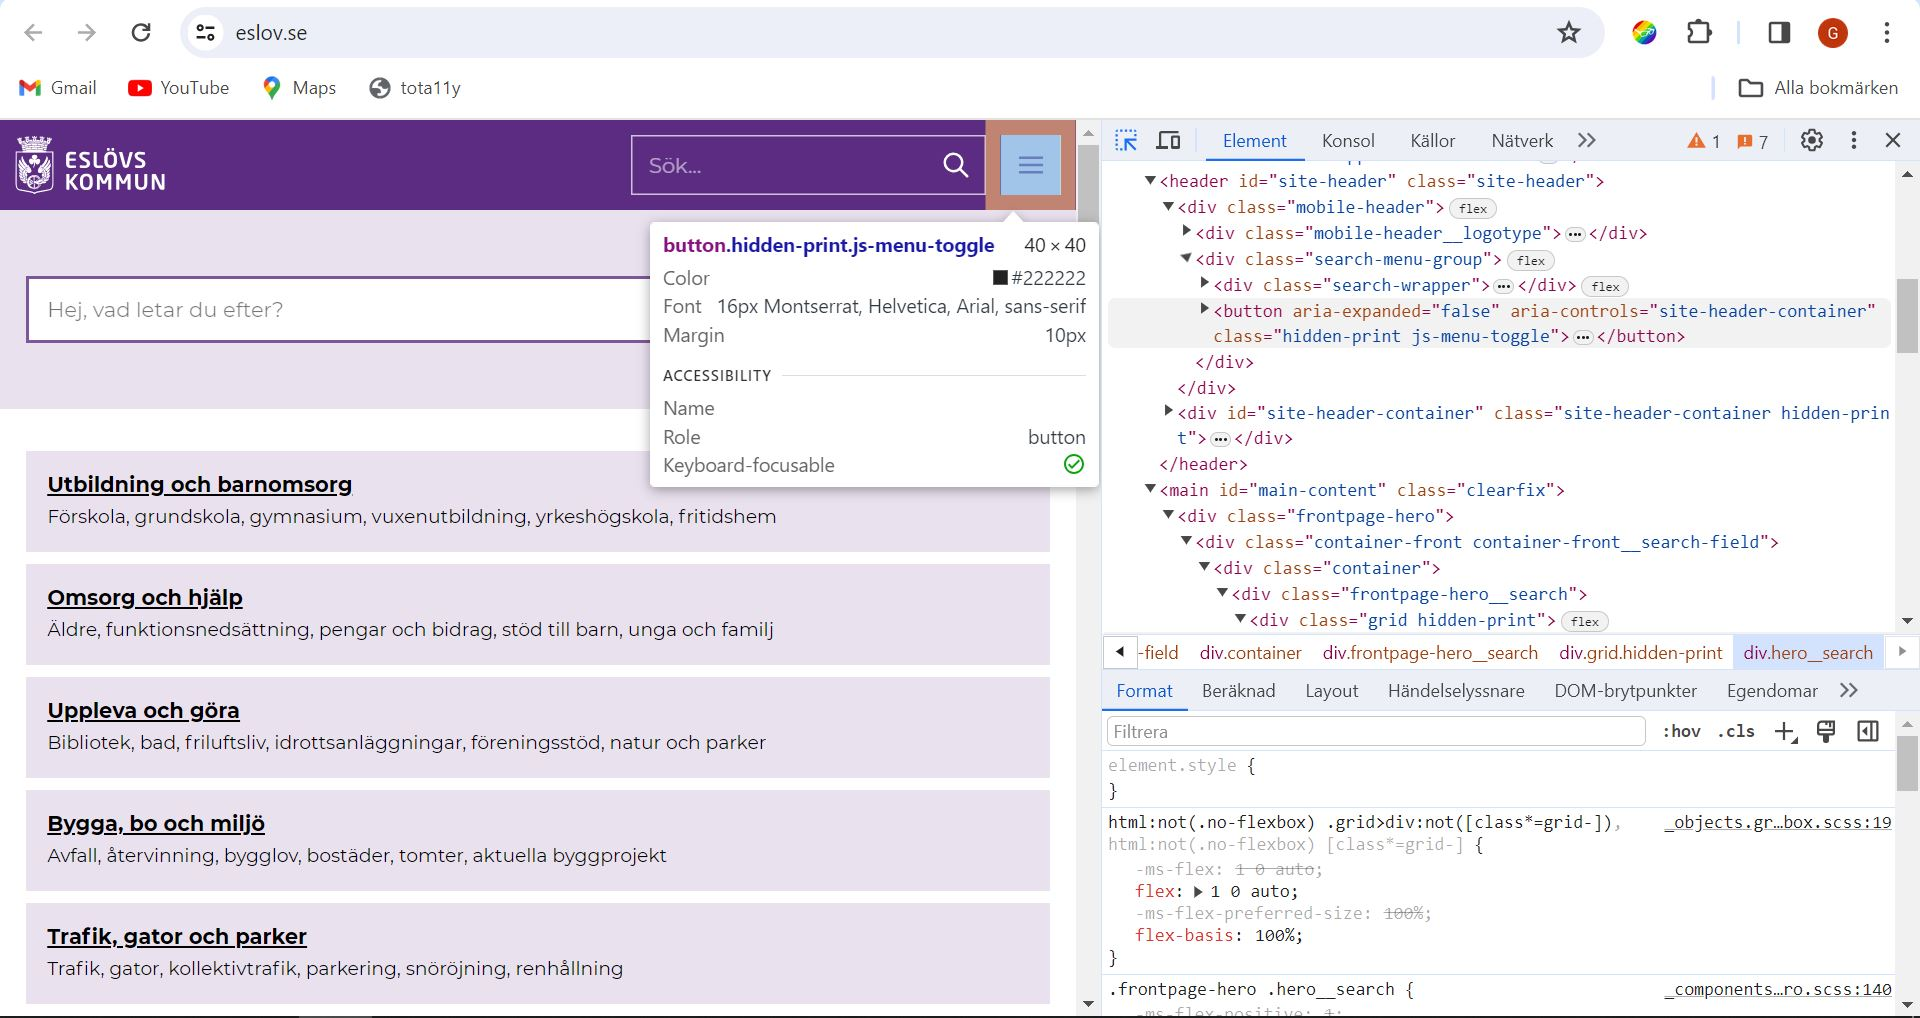
\includegraphics[width=0.8\textwidth]{../images/Eslov253.jpg}
        \caption{ Eslov.se med en knapp som inte har ett namn }
    \end{figure}

    \begin{figure}[hbt!]
        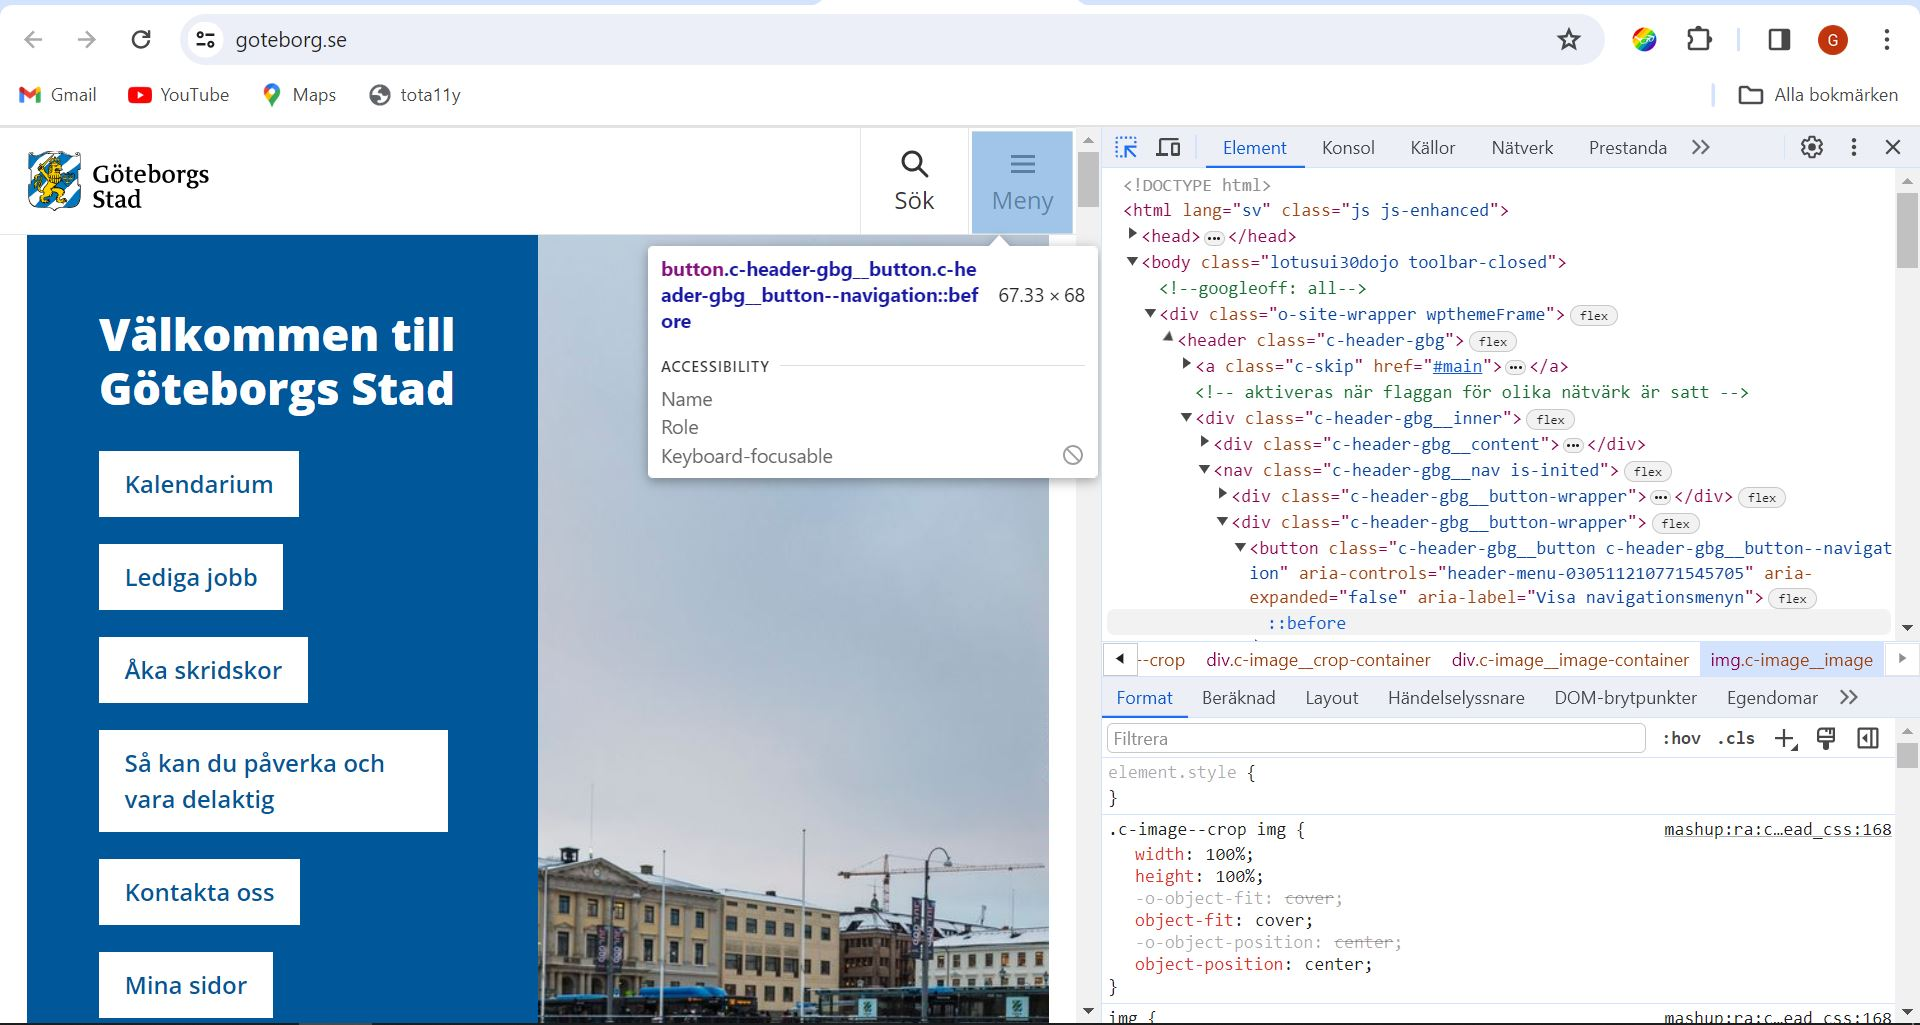
\includegraphics[width=0.8\textwidth]{../images/Goteborg253.jpg}
        \caption{ Goteborg.se med en knapp som inte har ett namn }
    \end{figure}

    \begin{figure}[hbt!]
        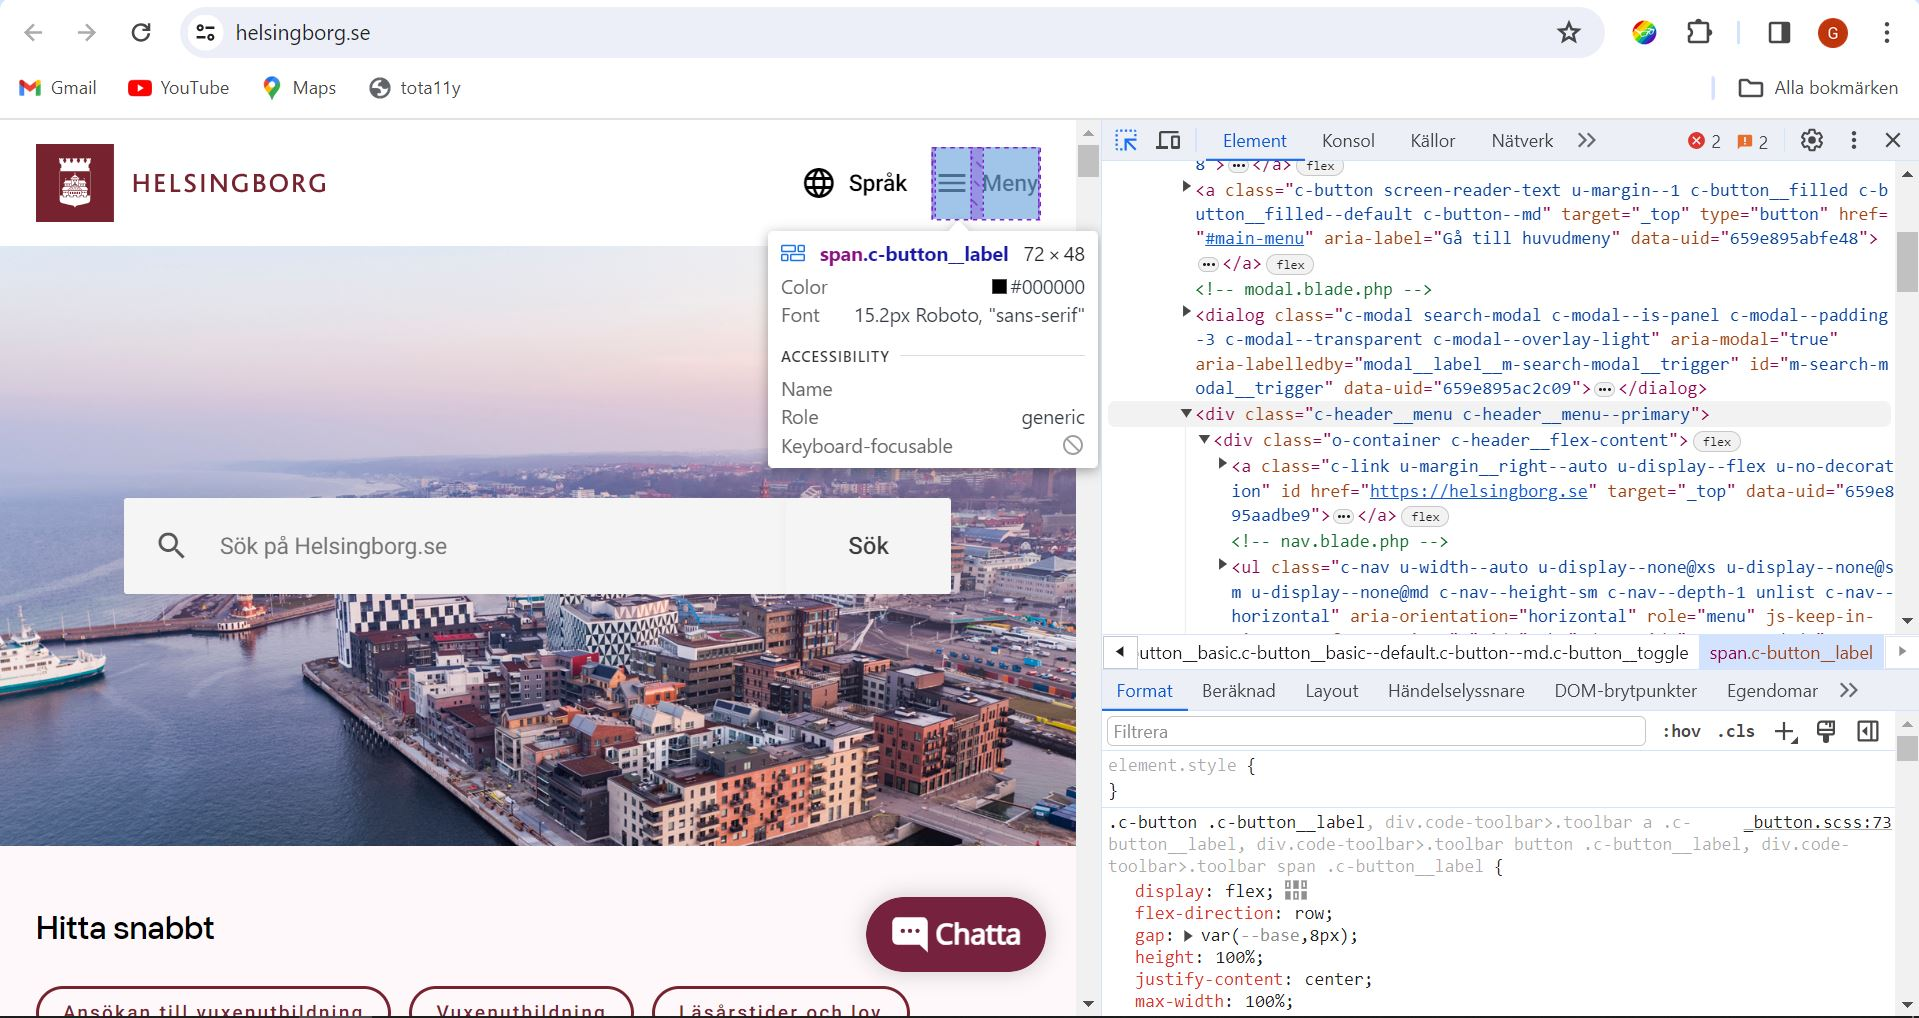
\includegraphics[width=0.8\textwidth]{../images/Helsingborg253.jpg}
        \caption{ Helsingborg.se med en knapp som inte har ett namn }
    \end{figure}
<
    \subsection{Lighthouse}

    Resultatet från Lighthouse testerna kommer att visa sidornas prestanda, tillgänglighet och hur de arbetar utifrån bästa praxis.
    Undersökningen resulterade i att alla webbsidor hade högt medelvärde i prestanda och praxis.
    Dock så hade goteborg.se och helsingborg.se betydligt lägre tillgänglighet ifall man jämför med resten av sidorna och detta syns i figur 11

    \begin{figure}[hbt!]
        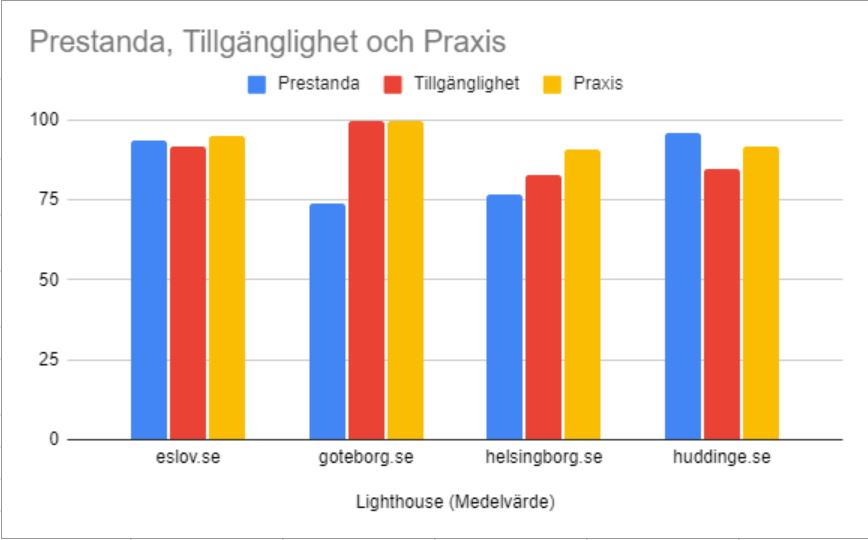
\includegraphics[width=0.8\textwidth]{../images/Medelvarde.jpg}
        \caption{ Medelvärdet på lighthouse testerna utfört på dator versionen }
    \end{figure}

    Webbsidorna med lägst medelvärde på tillgänglighet var goteborg.se och helsingborg.se som endast hade 74 respektive 77 poäng utav 100.
    Utöver det uppnådde de flesta webbsidorna över 80 poäng om inte mer på prestanda och praxis.
    Webbsidan med bäst lighthouse resultat på datorn är eslov.se.

    \section{Diskussion}
    Baserat på undersökningens frågeställning och det resultat som undersökningen framställde så vill jag diskutera delar av resultatet.
    Utifrån frågan om sidorna kunde uppfylla tillgänglighetskraven WCAG 2.1, var de flesta kraven uppfyllda utom några enstaka på alla webbsidor.
    Det var få krav som inte uppfylldes vilket var positivt överraskande.
    Alla webbsidor klarade inte av kriteriet 1.1.1 inom WCAG 2.0 vilket syns i figur [NUMMER].
    Alternativ text kan vara en enkel sak som många utvecklare av sidor kan missa eller inte uppfylls helt.
    Det finns program som kan användas för att förenkla denna process med att skriva alt-taggarna.
    Däremot är det också viktigt att nämna att det inte behöver vara utvecklarna av sidan som orsakade denna miss.
    Det kan vara den person som hanterar text eller innehåll på sidan som inte gav utvecklaren den alternativa texten som behövs.
    Webbsidor kan också använda sig utav att gömma denna typ av innehåll när skärmläsare skulle användas, dock så går det att argumentera om detta är en tillräckligt bra lösning på problemet.

    Den oroväckande trenden att webbsidorna inte klarar av att ha samma namn som sina input element som visas visuellt (kriterium 2.5.3).
    Kriteriet kräver att alla inmatningselement med text eller bild ska ha samma namn.
    Detta görs för att förenkla användningen av röstinmatning.
    Alla sidor förutom huddinge.se hade en del på sidan som inte klarade av detta kriteriet på olika sätt.
    Detta går även för kriteriet 1.1.1 och alla webbsidor som jag undersökt med alternativ text istället och detta väcker frågan om hur mycket detta faktiskt prioriteras.
    
    \section{Slutsatser}
    I det stora hela hittades få problem med webbsidorna och det var få kriterier som inte uppfylldes vilket var positivt.
    Däremot bör de problem som hittades förbättras för att få mer tillgängliga sidor.
    Förbättringar som skulle kunna göras för en liknande studie skulle kunna vara att använda sig utav nya WCAG 2.2 eller WCAG 3.0 som håller på att utvecklas fortfarande för att bli den nya webbstandarden.
    En djupare undersökning på webbsidornas olika sidor skulle även göra ett mer utförligt arbete.


    \printbibliography

\end{document}